\documentclass[letterpaper]{article}
\usepackage{fullpage}
\usepackage[table]{xcolor}
\usepackage{tabularx}
\usepackage{graphicx}
\usepackage{amsmath}
\usepackage{hyperref}
\usepackage{listings}
\lstset{language=python, tabsize=4}

\title{Deep Learning Approach to Link Weight Prediction}

\begin{document}
\maketitle


\section{Experiments}
We evaluate Model R experimentally
and the results show that 
Model R can achieve much lower prediction error than the baseline models \cite{aicher2014learning}.

\subsection{Datasets}
The experiments use 4 datasets summarized in \autoref{tab:datasets}.
\begin{table}[!htb]
	\centering
	\caption{The datasets used in experiments.}
	\begin{tabularx}{\textwidth}{|c|c|X|c|X|}  \hline \rowcolor{blue!50}
		Dataset & Node count & Node type & Link count & Link weight type \\ \hline
		Airport\cite{colizza2007reaction} & 500 & busiest airports in US & 5960 & number of passengers traveling from one airport to the other\\ \hline
		Collaboration\cite{pan2012world} & 226 & nations on Earth & 20616 & number of academic papers written by authors from the two connected nations \\ \hline
		Congress\cite{porter2005network} & 163  & 102nd US Congress committees & 26569 & interlock value of shared members from the two committees \\ \hline
		Forum\cite{opsahl2009clustering}  & 1899 & users of a student social network at UC Irvine & 20291 & number of messages sent from one student to the other \\ \hline
	\end{tabularx}
	\label{tab:datasets}
\end{table}

\subsection{Experiment process}
We do the same experiment for each dataset.
All the link weights are normalized to ranger [-1, 1] after applying a logarithm function.
Each experiment consists of 25 independent trials.
In each trial, we split the dataset randomly into 3 subsets:
\begin{itemize}
	\item 70\% into training set
	\item 10\% into validation set
	\item 20\% into testing set
\end{itemize}
We use mean squared error as the prediction accuracy metric.
For each experiment, we report the mean and standard deviation of the errors from 25 trials.
The pseudo code of the experiment process is as follows:

\begin{lstlisting}
	def main():
		for dataset in [Airport, Collaboration, Congress, Forum]:
			(error_mean, error_standard_deviation) = do_experiment(dataset)
	def do_experiment(dataset):
		errors = list()
		for trial in range(25):
			testing_error = append(evaluate_model_on(dataset))
			errors.append(testing_error)
		return (errors.mean(), errors.standard_deviation())
	def evaluate_model_on(dataset):
		(trainning_set, validation_set, testing_set) = split(dataset)
		while validation_error decreases:
			training_error = estimator.learn(training_set)
			validation_error = estimator.predict(validation_set)
		testing_error = estimator.predict(testing_set)
		return testing_error
\end{lstlisting}

\subsection{Experiment results}
In our experiments,
Model R's error is lower than every other model on every dataset,
shown in \autoref{fig:errors}.
\begin{figure}[!htb]
	\centering
	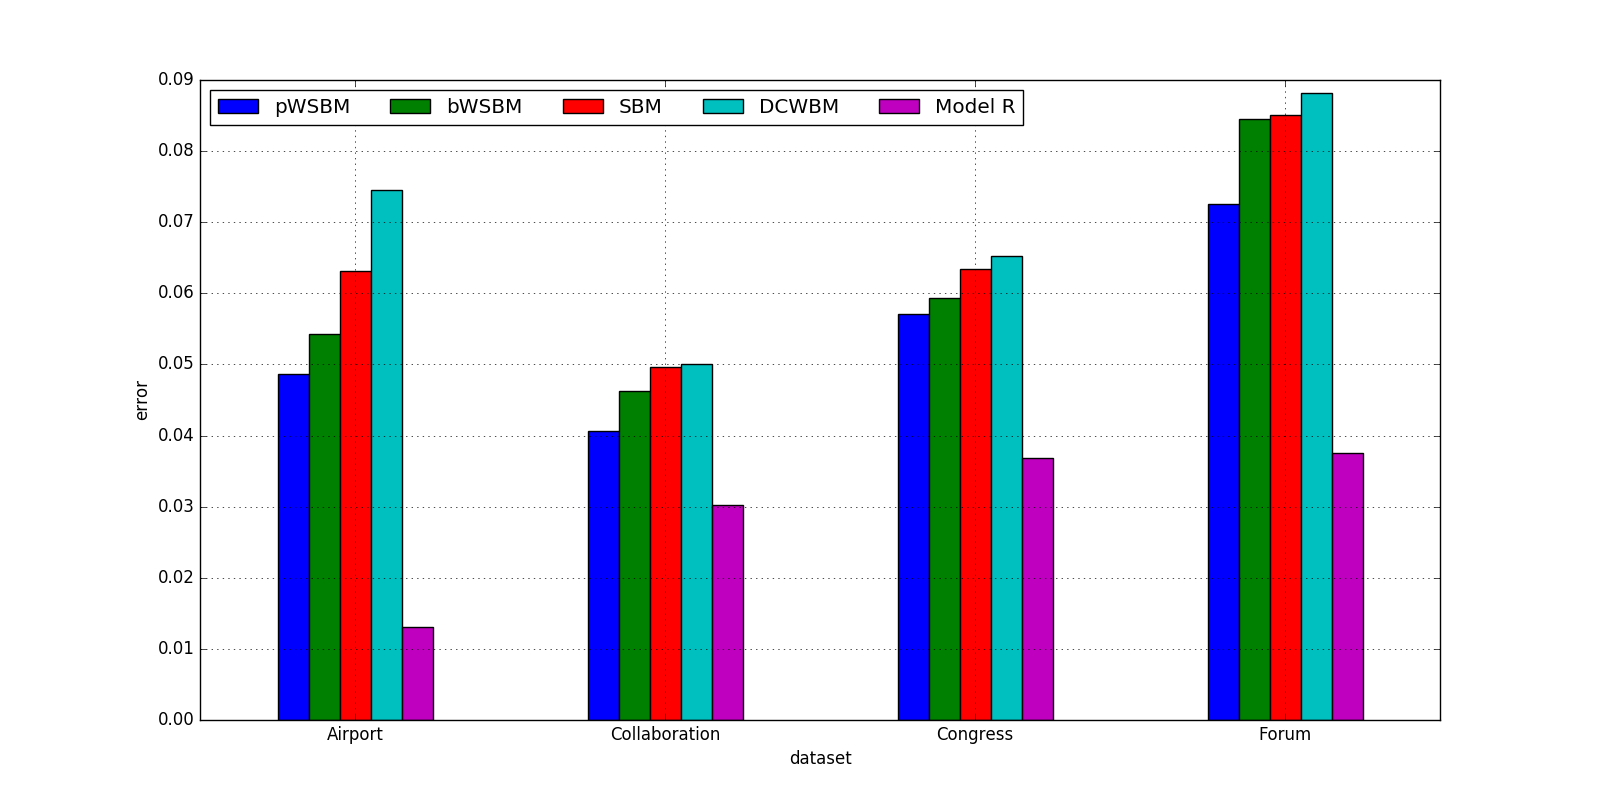
\includegraphics[width=\textwidth]{link-weight-errors}
	\caption[content...]{
		The mean squared errors of 5 models on 4 datasets:
		Model R has lower error than every other model on every dataset.
		Every error value shown here is the mean errors for the 25 trials in the experiment.
	}
	\label{fig:errors}
\end{figure}
For this section we compare Model R with only the best baseline model - pWSBM, as it outperforms other baseline models on every dataset.
Given the dataset, we regard ModelRError (or BaselineError) as a random variable so each trial generates an example of it.
We can do a t-test to justify the significance of difference between the means of variables ModelRError and BaselineError.
where $ \overline{X} $ is the mean of variable X.
The mean of a variable is not the same as the mean of a sample of the variable.
More specifically,
a variable can generate two samples with different sample means,
therefore two different sample means does not imply the two variables generating them have different means.
For each dataset, we do a t-test for the two variables where the null hypothesis is that the two variables have the same mean:
\begin{align*}
\overline{X_1} == \overline{X_2}
\end{align*}
where $ X_1 $ and $ X_2 $ are ModelRError and BaselineError.
The standard deviation $ s $ of variable X is defined as:
\begin{align*}
	s_i &= \sqrt{\overline{(X_i - \overline{X_i})^2}}
\end{align*}
Welch's t-test defines its statistic t and degrees of freedom v as:
\begin{align*}
	t &= \frac{
		\overline{X_1} - \overline{X_2}
		}{
		\sqrt{\frac{s^2_1}{N_1} + \frac{s^2_2}{N_2}}
		}\\
	v &= \frac{
		(\frac{s^2_1}{N_1} + \frac{s^2_2}{N_2})^2
		}{
		\frac{s^4_1}{N_1^2(N_1-1)} + \frac{s^4_2}{N_2^2(N_2-1)}
		}
\end{align*}
where $ N_i $ is the sample size of variable $ X_i $.
The Student's t-distribution defines its probability density function f(x) as:
\begin{align*}
f(x) = \frac{\Gamma(\frac{v+1}{2})}{\sqrt{v\pi}\Gamma(\frac{v}{2})}
((1+\frac{x^2}{v})^{-\frac{v+1}{2}})
\end{align*}
Welch's t-test defines its p value as the Student's t-distribution cumulative density function:
\begin{align*}
p = 2 \int_{-\infty}^{-|t|} f(x) dx
\end{align*}
The smaller p is, the more confidently we can reject the null hypothesis, i.e., accept that:
\begin{align*}
\overline{ModelRError} \neq \overline{BaselineError}
\end{align*}
Typically there is a domain specific threshold for p, e.g., 0.1 or 0.01. If p is smaller than the threshold we reject the null hypothesis.
We calculate the p value and also error reduction from baseline to Model R as:
\begin{align*}
Reduction = \frac{BaselineError - ModelRError}{BaselineError}
\end{align*}
The p value is almost 0 for all datasets and error reduction is significant:
ranging from 25\% on Collaboration dataset to 73\% on Airport dataset,
shown in \autoref{tab:errors}.
\begin{table}[!htb]
	\centering
	\caption{
		The mean squared errors of 5 models on 4 datasets:
		Model R has lower error than every other model on every dataset,
		reducing error by 25\% to 73\% from the best baseline model - pWSBM.
		The number in every parenthesis is the standard deviation of error in 25 trials in the last digit of error. The very low p values strongly indicate the error reduction is significant.
	}
	\begin{tabularx}{\textwidth}{|X|c|c|c|c|c|c|c|} \hline \rowcolor{blue!50}
		Dataset & pWSBM & bWSBM & SBM & DCWBM & Model R & Reduction & p \\ \hline
		Airport & 0.0486(6) & 0.0543(5) & 0.0632(8) & 0.0746(9) & 0.013(1) & 73\% & 4.2e-66 \\ \hline
		Collaboration & 0.0407(1) & 0.0462(1) & 0.0497(3) & 0.0500(2) & 0.030(1) & 25\% & 9.1e-44 \\ \hline
		Congress & 0.0571(4) & 0.0594(4) & 0.0634(6) & 0.0653(4) & 0.036(3) & 35\% & 7.1e-35 \\ \hline
		Forum & 0.0726(3) & 0.0845(3) & 0.0851(4) & 0.0882(4) & 0.037(1) & 48\% & 4.2e-68 \\ \hline
	\end{tabularx}
	\label{tab:errors}
\end{table}
These results show that Model R outperforms pWSBM on all these datasets.

\subsection{Computing resources}
We ran our experiments on a Lenovo ThinkCentre M83 machine with the following specifications:
\begin{itemize}
	\item Python implementation: CPython 3.5
	\item Operating system: Ubuntu 16.10 64-bit
	\item Memory: 16 GB
	\item Processor: Intel Core i7-4770 CPU @ 3.40GHz $ \times $ 8
\end{itemize}
The program - coded in Python - uses all 8 threads of the processor.
Each experiment takes about one hour to finish,
depending on the dataset and parameters in the learning algorithm.

\bibliographystyle{plain}
\bibliography{references}
\end{document}
